\documentclass{beamer}
% imprimir
% \documentclass[handout]{beamer} 
% \usepackage{pgfpages}
% \pgfpagesuselayout{4 on 1}[a4paper,landscape,border shrink=5mm]

\mode<presentation> {
  \usetheme{Warsaw}
  \setbeamercovered{transparent}
}

\usebackgroundtemplate{
\includegraphics[width=\paperwidth]{format/libresoft-bg.png}}
\usepackage[spanish]{babel}
\usepackage[utf8]{inputenc}
\usepackage{graphics}
\usepackage{amssymb} % Simbolos matematicos

%\definecolor{libresoftgreen}{RGB}{162,190,43}
%\definecolor{libresoftblue}{RGB}{0,98,143}

%\setbeamercolor{titlelike}{bg=libresoftgreen}

%% Metadatos del PDF.
\hypersetup{  
  pdftitle={Training and Certifications},
  pdfauthor={Pedro Coca},
  pdfcreator={GSyC/Libresoft},
  pdfproducer=PDFLaTeX,
  pdfsubject={Systems Security},
}
%%

\begin{document}

\title{Training and Education}
\subtitle{Arquitectura de servidores con software libre}
\institute{pcoca@libresoft.es} 
\author{Pedro Coca}
%\date{\today}
\date{27th May 2011}

\frame{
\maketitle
\begin{center}

\includegraphics[width=6cm]{format/gsyc-urjc}
\end{center}
}

\frame{
~
\vspace{4cm}

\begin{flushright}
{\small
(cc) 2011 Pedro Coca. \\
  This presentation is publised under the Creative Commons 3.0 Attribution, available at 
  \url{http://creativecommons.org/licenses/by/3.0/}
 

\bigskip

}
\end{flushright}
}
%%

\section{Training and Education: Introduction}

\begin{frame}
\frametitle{Introduction}
\begin{itemize}
\item IT Certifications
\item Certifications and Job Market analysis
\item Certifications and Competence
\item Training and educational needs (Spanish SME)
\end{itemize}
\end{frame}

%%%%%%%%%%%%%%%%%%%%%%%%%%%%%%%%%%%%%%%%%%%%%%%%%%%%%%%%%%%%

\section{IT Certifications}

%%%%%%%%%%%%%%%%%%%%%%%%%%%%%%%%%%%%%%%%%%%%%%%%%%%%%%%%%%%%

\begin{frame}
\frametitle{IT Certification Introduction}
\begin{itemize}
\item The value of an IT certification
\item Very Industry-oriented
\item Sometimes very Vendor-oriented!
\item IT Certifications article at BSD Magazine:
\begin{itemize}
\item October 2010 Issue
\item \url{https://samzplace.wordpress.com/2010/10/}
\item \url{http://bsdmag.org/system/articles/attachment1s/12805/original/VPN_and_BSD_BSD_10_2010.pdf}
\end{itemize}
\end{itemize}
\end{frame}


%%%%%%%%%%%%%%%%%%%%%%%%%%%%%%%%%%%%%%%%%%%%%%%%%%%%%%%%%%%%


\begin{frame}
\frametitle{IT Certification List}
\begin{itemize}
\item {\bf ISACA}: CISA and CISM
\item {\bf ISC2}: CISSP
\item {\bf EC-Council}: CEH
\item {\bf LPI}: Linux Professional Institute Series
\item {\bf Red Hat}: RHCE and RHCSA
\item {\bf Sun}: Sun Certified ... 
\item {\bf Cisco}: Cisco Certified ... (CCNA, CCNP, etc)
\item {\bf Canonical}: Ubuntu Certified Professional
\end{itemize}
\end{frame}

%%%%%%%%%%%%%%%%%%%%%%%%%%%%%%%%%%%%%%%%%%%%%%%%%%%%%%%%%%%%

\begin{frame}
\frametitle{ISACA}
\begin{itemize}
\item {\bf ISACA}: Information Systems Audit and Control Association
\item International professional association
\item Not just Audit and Control
\item IT Governance oriented
\item Founded in USA in 1967
\item More than 95,000 constituents 
\item More than 160 countries
\item Published many reference books about Governance, IT Risk Management, etc
\item \url{http://www.isaca.org}
\end{itemize}
\end{frame}

%%%%%%%%%%%%%%%%%%%%%%%%%%%%%%%%%%%%%%%%%%%%%%%%%%%%%%%%%%%%

\begin{frame}
\frametitle{ISACA Certifications}
\begin{itemize}
\item Certified Information Systems Auditor (CISA)
\item Certified Information Security Manager (CISM)
\item Certified in the Governance of Enterprise IT (CGEIT)
\item Certified in Risk and Information Systems Control (CRISC)
\end{itemize}
\end{frame}


%%%%%%%%%%%%%%%%%%%%%%%%%%%%%%%%%%%%%%%%%%%%%%%%%%%%%%%%%%%%

\begin{frame}
\frametitle{CISA}
\begin{itemize}
\item Certified Information Security Auditor
\item Established in 1978
\item Over 79,000 CISAs in 2010
\item Formally approved by the US Department of Defense (Information Assurance Technical category)
\item Changing in 2011
\item 5 years of experience required (there are some waivers)
\end{itemize}
\end{frame}


%%%%%%%%%%%%%%%%%%%%%%%%%%%%%%%%%%%%%%%%%%%%%%%%%%%%%%%%%%%%


\begin{frame}
\frametitle{CISA Exam}
\begin{itemize}
\item Exam Domains
\begin{itemize}
\item The Process of Auditing Information Systems
\item Governance and Management of IT
\item Information Systems Acquisition, Development and Implementation
\item Information Systems Operations, Maintenance and Support
\item Protection of Information Assets
\end{itemize}
\item 200 Questions. Score range: 200-800. (450 needed to pass)
\item Offered in 12 languages at more than 200 locations worldwide
\item Just in June and December
\item 4 Hours
\item Passing the exam does not mean to be certified!
\end{itemize}
\end{frame}


%%%%%%%%%%%%%%%%%%%%%%%%%%%%%%%%%%%%%%%%%%%%%%%%%%%%%%%%%%%%

\begin{frame}
\frametitle{CISM}
\begin{itemize}
\item Certified Information Security Manager
\item Continues CISA path
\item More managerial certification
\item Also formally approved by the US Department of Defense
\item 5 years of experience required. 3 years of Managing experience
\end{itemize}
\end{frame}

%%%%%%%%%%%%%%%%%%%%%%%%%%%%%%%%%%%%%%%%%%%%%%%%%%%%%%%%%%%%


\begin{frame}
\frametitle{CISM Exam}
\begin{itemize}
\item Exam Domains
\begin{itemize}
    \item Information Security Governance
    \item Information risk management
    \item Information security program development
    \item Information security program management
    \item Incident management
\end{itemize}
\item 200 Questions. Score range: 200-800. (450 needed to pass)
\item Offered in 12 languages at more than 200 locations worldwide
\item Just in June and December
\item 4 Hours
\item Passing the exam does not mean to be certified!
\end{itemize}
\end{frame}

%%%%%%%%%%%%%%%%%%%%%%%%%%%%%%%%%%%%%%%%%%%%%%%%%%%%%%%%%%%%

\begin{frame}
\frametitle{ISC2}
\begin{itemize}
\item International Information Systems Security Certification Consortium
\item Non-profit organization based in Florida (USA)
\item Established in 1989
\item Goal: Set a standardized certification program that provided structure and demonstrated competence
\item \url{https://www.isc2.org/}
\end{itemize}
\end{frame}

%%%%%%%%%%%%%%%%%%%%%%%%%%%%%%%%%%%%%%%%%%%%%%%%%%%%%%%%%%%%%

\begin{frame}
\frametitle{ISC2 Certifications}
\begin{itemize}
    \item Certified Information Systems Security Professional (CISSP)
    \item Information Systems Security Architecture Professional (ISSAP)
    \item Information Systems Security Management Professional (ISSMP)
    \item Information Systems Security Engineering Professional (ISSEP)
    \item Certification and Accreditation Professional (CAP)
    \item Systems Security Certified Practitioner (SSCP)
    \item Certified Secure Software Lifecycle Professional (CSSLP)
\end{itemize}
\end{frame}

%%%%%%%%%%%%%%%%%%%%%%%%%%%%%%%%%%%%%%%%%%%%%%%%%%%%%%%%%%%

\begin{frame}
\frametitle{CISSP}
\begin{itemize}
    \item Certified Information Systems Security Professional (CISSP)
    \item 67.744 CISSP in 134 countries (July 2010)
    \item First information security ANSI ISO/IEC credential 
       \begin{itemize}
       \item June 2004 
       \item Standard 17024:2003
       \end{itemize}
    \item Formally approved by the U.S. Department of Defense (DoD)
       \begin{itemize}
       \item Information Assurance Technical (IAT) 
       \item Managerial (IAM) 
       \end{itemize}
    \item Baseline for the US National Security Agency's ISSEP
\end{itemize}
\end{frame}

%%%%%%%%%%%%%%%%%%%%%%%%%%%%%%%%%%%%%%%%%%%%%%%%%%%%%%%%%%%%

\begin{frame}
\frametitle{CISSP Domains}
\begin{itemize}
    \item Access Control Systems and Methodology
    \item Telecommunications and Network Security
    \item Business Continuity Planning and Disaster Recovery Planning
    \item Security Management Practices
    \item Security Architecture and Models
    \item Law, Investigation, and Ethics
    \item Application and Systems Development Security
    \item Cryptography
    \item Computer Operations Security
    \item Physical Security
\end{itemize}
\end{frame}

%%%%%%%%%%%%%%%%%%%%%%%%%%%%%%%%%%%%%%%%%%%%%%%%%%%%%%%%%%%%

\begin{frame}
\frametitle{CISSP Exam}
\begin{itemize}
    \item 250 test questions
    \item 6 Hours
    \item On demand / Concentration venues
    \item Valid for only three years, after which it must be renewed
    \item 25 test questions are for research purposes
\end{itemize}
\end{frame}

%%%%%%%%%%%%%%%%%%%%%%%%%%%%%%%%%%%%%%%%%%%%%%%%%%%%%%%%%%%%

\begin{frame}
\frametitle{CISSP reputation damage}
\begin{center}
   \huge {Samsung keylogger software issue}
\end{center}
\end{frame}

%%%%%%%%%%%%%%%%%%%%%%%%%%%%%%%%%%%%%%%%%%%%%%%%%%%%%%%%%%%%

\begin{frame}
\frametitle{CISSP reputation damage}
\begin{itemize}
    \item March 2011
    \item Samsung Keylogging
    \item Poorly investigated by a CISSP
    \item Samsung reputation has been damaged
    \item CISSP reputation has also been damaged
\end{itemize}
\end{frame}

%%%%%%%%%%%%%%%%%%%%%%%%%%%%%%%%%%%%%%%%%%%%%%%%%%%%%%%%%%%%%

\begin{frame}
\frametitle{Certified Ethical Hacker}
\begin{itemize}
\item International Council of E-Commerce Consultants (EC-Council.) 
\item Very focused on Security and Pen-test
\item 2 years of experience needed in security industry
\end{itemize}
\end{frame}


%%%%%%%%%%%%%%%%%%%%%%%%%%%%%%%%%%%%%%%%%%%%%%%%%%%%%%%%%%%%

\begin{frame}
\frametitle{Linux Professional Institute}
\begin{itemize}
\item Non-profit organization 
\item Provides vendor-independent professional certification
\item Aimed to Linux system administrators and programmers
\item Founded in 1999 (Canada)
\end{itemize}
\end{frame}

%%%%%%%%%%%%%%%%%%%%%%%%%%%%%%%%%%%%%%%%%%%%%%%%%%%%%%%%%%%%%

\begin{frame}
\frametitle{LPI Certifications}
\begin{itemize}
\item LPIC - Level 1
    \begin{itemize}
    \item Junior Level Administration
    \item First published 2000 
    \item 101 and 102 exams
    \end{itemize}
\item LPIC - Level 2
    \begin{itemize}
    \item Advanced Level Administration
    \item First published 2001 
    \item 201 and 202 exams
    \end{itemize}
\item LPIC - Level 3
    \begin{itemize}
    \item Senior Level Administration
    \item First published 2007 
    \item 301 and 302 exams
    \end{itemize}
\end{itemize}
\end{frame}

%%%%%%%%%%%%%%%%%%%%%%%%%%%%%%%%%%%%%%%%%%%%%%%%%%%%%%%%%%%%

\begin{frame}
\frametitle{Vendor Specific Certifications}
\begin{itemize}
\item Provides vendor-dependent training
\item Aimed to specific technologies and narrowed down fields
\item Industrial agents
\begin{itemize}
    \item Sun (Oracle) 
    \item Cisco 
    \item Canonical 
    \item Red Hat
    \item ...
\end{itemize}
\item CCNA, CCNP, RHCSA, RHCE, Ubuntu Certified Professional, Sun Certified...
\end{itemize}
\end{frame}


%%%%%%%%%%%%%%%%%%%%%%%%%%%%%%%%%%%%%%%%%%%%%%%%%%%%%%%%%%%%

\section{Certification and Job Market Analysis}

%%%%%%%%%%%%%%%%%%%%%%%%%%%%%%%%%%%%%%%%%%%%%%%%%%%%%%%%%%%%

\begin{frame}
\frametitle{Certification and Job Market Analysis}
\begin{itemize}
\item Let's search on-line for job opportunities

\item Which job search sites? 
  \begin{itemize}
  \item Local ones, aimed to spanish market
  \item A couple of US job search sites
  \end{itemize}

\item This analysis was carried out in April 2011

\item Please take into consideration: 
  \begin{itemize}
  \item Spanish and US job market situations and sizes
  \item Economic contexts
  \item It is not a comprehensive market research
  \end{itemize}

\end{itemize}
\end{frame}


%%%%%%%%%%%%%%%%%%%%%%%%%%%%%%%%%%%%%%%%%%%%%%%%%%%%%%%%%%%%

\begin{frame}
\frametitle{Certification and Job Market Analysis}
\begin{itemize}

\item Spanish market job search engines
  \begin{itemize}
  \item infojobs.net
  \item tecnoempleo.com	
  \item infoempleo.com	
  \item laboris.net
  \item monster.es
  \end{itemize}

\item US market job search engines
  \begin{itemize}
  \item careerbuilder.com
  \item dice.com
  \end{itemize}

\end{itemize}

\end{frame}

%%%%%%%%%%%%%%%%%%%%%%%%%%%%%%%%%%%%%%%%%%%%%%%%%%%%%%%%%%%%

\begin{frame}
\frametitle{IT Certifications search: infojobs.net}
\begin{center}
  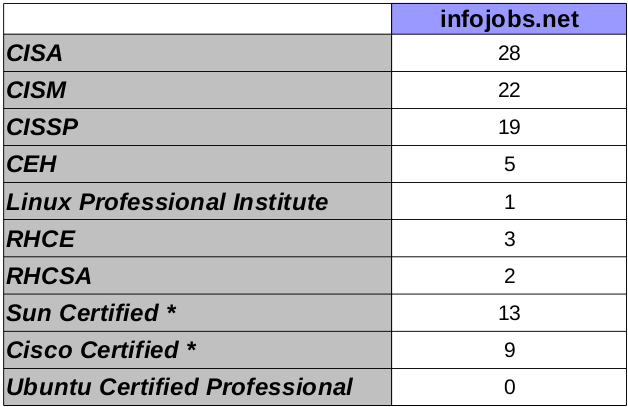
\includegraphics[width=8cm]{figs/infojobs.png}
\end{center}
\begin{center}
\normalsize{32725 Job positions offered. April 2011}
\end{center}
\end{frame}

%%%%%%%%%%%%%%%%%%%%%%%%%%%%%%%%%%%%%%%%%%%%%%%%%%%%%%%%%%%%

\begin{frame}
\frametitle{IT Certifications search: tecnoempleo.com}
\begin{center}
  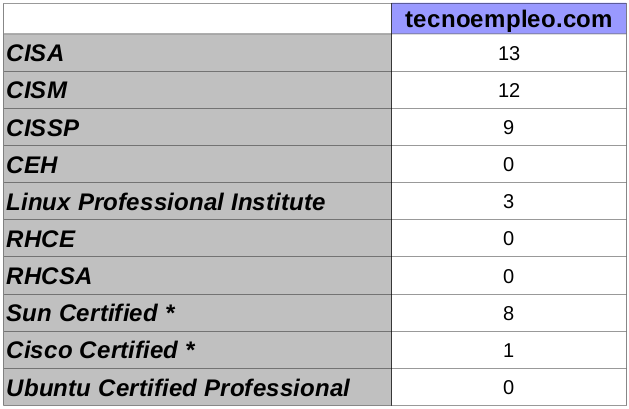
\includegraphics[width=8cm]{figs/tecnoempleo.png}
\end{center}
\begin{center}
\normalsize{6951 Job positions offered. April 2011}
\end{center}
\end{frame}


%%%%%%%%%%%%%%%%%%%%%%%%%%%%%%%%%%%%%%%%%%%%%%%%%%%%%%%%%%%%

\begin{frame}
\frametitle{IT Certifications search: infoempleo.com}
\begin{center}
  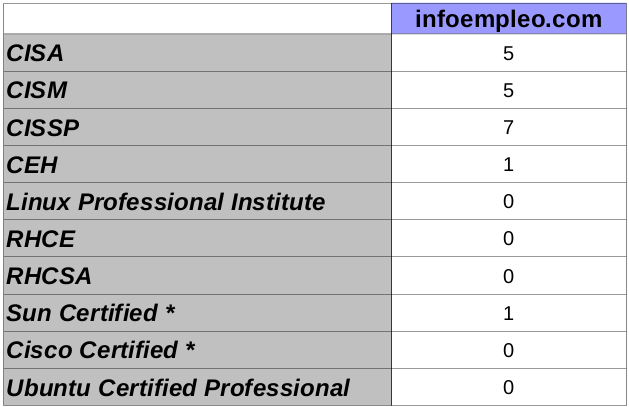
\includegraphics[width=8cm]{figs/infoempleo.png}
\end{center}
\begin{center}
\normalsize{10194 Job positions offered. April 2011}
\end{center}
\end{frame}


%%%%%%%%%%%%%%%%%%%%%%%%%%%%%%%%%%%%%%%%%%%%%%%%%%%%%%%%%%%%

\begin{frame}
\frametitle{IT Certifications search: laboris.net}
\begin{center}
  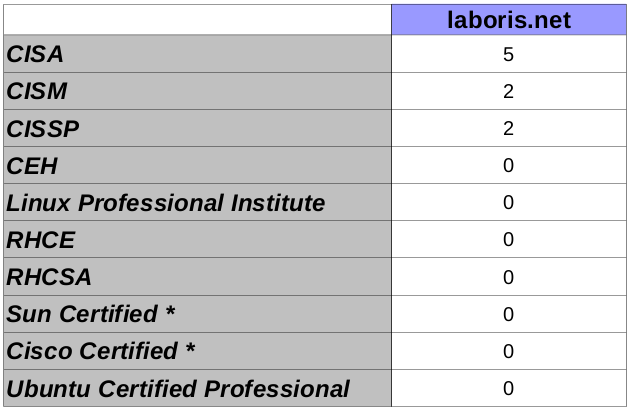
\includegraphics[width=8cm]{figs/laboris.png}
\end{center}
\begin{center}
\normalsize{No info about total job positions offered}
\end{center}
\end{frame}


%%%%%%%%%%%%%%%%%%%%%%%%%%%%%%%%%%%%%%%%%%%%%%%%%%%%%%%%%%%%

\begin{frame}
\frametitle{IT Certifications search: monster.es}
\begin{center}
  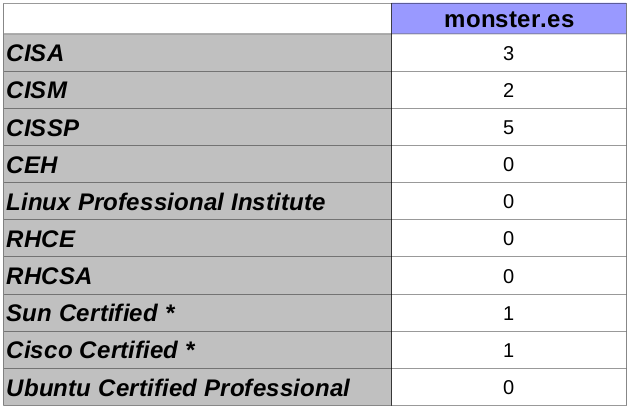
\includegraphics[width=8cm]{figs/monster.png}
\end{center}
\begin{center}
\normalsize{2329 Job positions offered. April 2011}
\end{center}
\end{frame}


%%%%%%%%%%%%%%%%%%%%%%%%%%%%%%%%%%%%%%%%%%%%%%%%%%%%%%%%%%%%

\begin{frame}
\frametitle{IT Certifications search: careerbuilder.com}
\begin{center}
  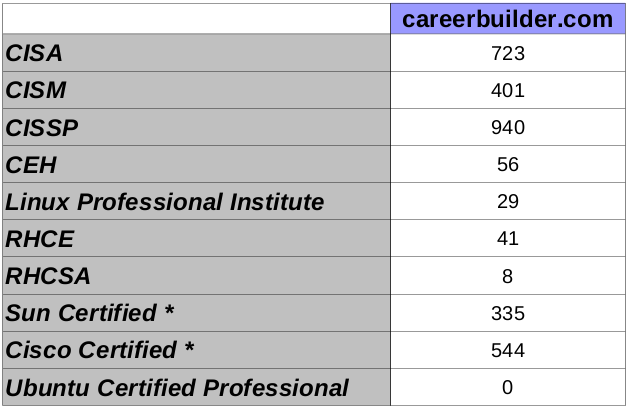
\includegraphics[width=8cm]{figs/careerbuilder.png}
\end{center}
\begin{center}
\normalsize{More than 100000 Job positions offered. April 2011}
\end{center}
\end{frame}


%%%%%%%%%%%%%%%%%%%%%%%%%%%%%%%%%%%%%%%%%%%%%%%%%%%%%%%%%%%%

\begin{frame}
\frametitle{IT Certifications search: dice.com}
\begin{center}
  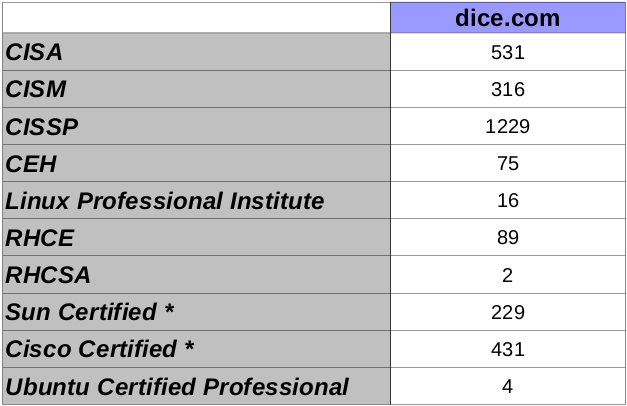
\includegraphics[width=8cm]{figs/dice.png}
\end{center}
\begin{center}
\normalsize{75594 Job positions offered. April 2011}
\end{center}
\end{frame}

%%%%%%%%%%%%%%%%%%%%%%%%%%%%%%%%%%%%%%%%%%%%%%%%%%%%%%%%%%%%

\begin{frame}
\frametitle{Questions? / Comments?}
\begin{center}
\huge{Questions? / Comments?}
\end{center}
\end{frame}

%%%%%%%%%%%%%%%%%%%%%%%%%%%%%%%%%%%%%%%%%%%%%%%%%%%%%%%%%%%%

\section{Certification and Competence}

%%%%%%%%%%%%%%%%%%%%%%%%%%%%%%%%%%%%%%%%%%%%%%%%%%%%%%%%%%%%

\begin{frame}
\frametitle{Certification and Competence}
\begin{itemize}
\item Do you think is there any correlation?
    \begin{itemize}
    \item Do the employers/market appreciate certifications?
    \item Is there any geographical/cultural deviation with the certifications?
    \end{itemize}
\item Certification-Competence Correlation Article
    \begin{itemize}
    \item \url{http://martinfowler.com/bliki/CertificationCompetenceCorrelation.html}
    \end{itemize}
\end{itemize}

\begin{center}
\huge{Lets discuss a little bit!}
\end{center}

\end{frame}

%%%%%%%%%%%%%%%%%%%%%%%%%%%%%%%%%%%%%%%%%%%%%%%%%%%%%%%%%%%%

\begin{frame}
\frametitle{Certification and Competence Correlation} 
\begin{center}
  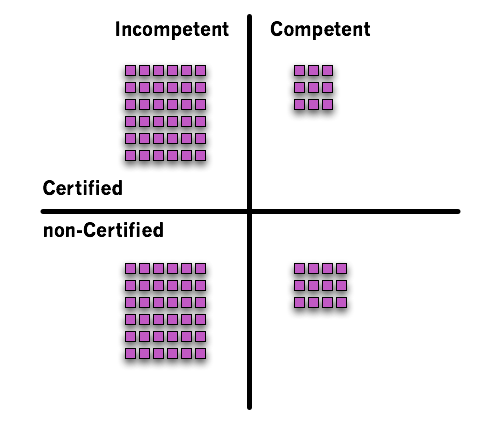
\includegraphics[width=5cm]{figs/CertificationCompetence.png}
\end{center}
\begin{center}
  \small{Martin Fowler Article. March 2011}
\end{center}
\end{frame}



%%%%%%%%%%%%%%%%%%%%%%%%%%%%%%%%%%%%%%%%%%%%%%%%%%%%%%%%%%%%


\begin{frame}
\frametitle{Questions? / Comments?}
\begin{center}
\huge{Questions? / Comments?}
\end{center}
\end{frame}

%%%%%%%%%%%%%%%%%%%%%%%%%%%%%%%%%%%%%%%%%%%%%%%%%%%%%%%%%%%%

\section{Educational and Training Needs: CENATIC Report}

%%%%%%%%%%%%%%%%%%%%%%%%%%%%%%%%%%%%%%%%%%%%%%%%%%%%%%%%%%%%


\begin{frame}
\frametitle{Educational and Training needs}
\begin{itemize}
\item CENATIC performed a deep study about the status of FLOSS in Spain
\item A report with the results was released in 2010 (CC-BY-3.0)
\item Several areas were covered
\item There was a specific area about training and educational needs
\item Helful information for Head of IT roles 
\end{itemize}
\end{frame}

%%%%%%%%%%%%%%%%%%%%%%%%%%%%%%%%%%%%%%%%%%%%%%%%%%%%%%%%%%%%

\begin{frame}
\frametitle{Issues finding FLOSS trained professionals: areas}
\begin{itemize}
\item Companies come across difficulties in findind educated and trained professionals in FLOSS
\item SMEs have more issues than big companies (FLOSS adoption is bigger in SMEs)
\item Biggest issues are usually found in business-related areas
   \begin{itemize}
   \item Security
   \item Integration
   \item Middleware
   \item Business Application
   \end{itemize}
\end{itemize}
\end{frame}

%%%%%%%%%%%%%%%%%%%%%%%%%%%%%%%%%%%%%%%%%%%%%%%%%%%%%%%%%%%%

\begin{frame}
\frametitle{Issues finding FLOSS trained professionals: areas}
\begin{center}
  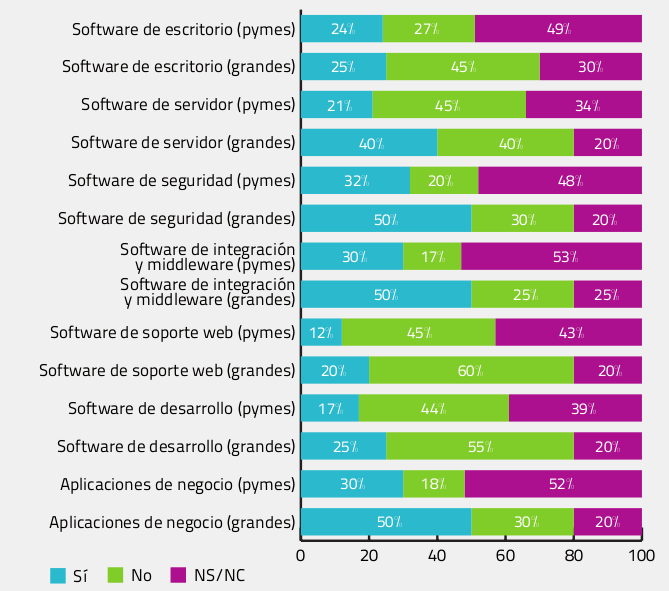
\includegraphics[width=6cm]{figs/cenatic_trainedprofessionals.png}
\end{center}
\end{frame}

%%%%%%%%%%%%%%%%%%%%%%%%%%%%%%%%%%%%%%%%%%%%%%%%%%%%%%%%%%%%

\begin{frame}
\frametitle{Internal Training}
\begin{itemize}
\item Companies with their businesses based on FLOSS
\item SMEs internal training activities is less than big companies
\item Relevant baseline of FLOSS trained professionals
\end{itemize}
\end{frame}

%%%%%%%%%%%%%%%%%%%%%%%%%%%%%%%%%%%%%%%%%%%%%%%%%%%%%%%%%%%%

\begin{frame}
\frametitle{Internal Training figures}
\begin{center}
  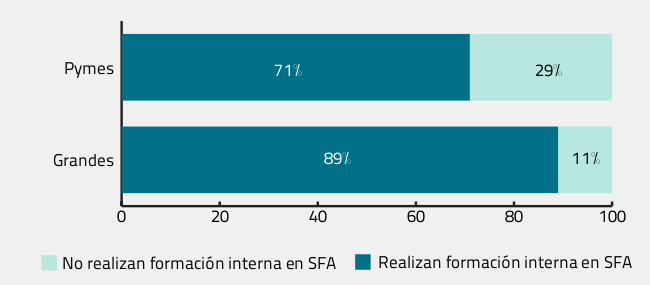
\includegraphics[width=8cm]{figs/cenatic_internaltraining.png}
\end{center}
\end{frame}

%%%%%%%%%%%%%%%%%%%%%%%%%%%%%%%%%%%%%%%%%%%%%%%%%%%%%%%%%%%%

\begin{frame}
\frametitle{Training budget}
\begin{itemize}
\item SMEs internal training activities is less than big companies
\item But SMEs invest a more significant percentage of training in FLOSS training
\item Big companies usually include privative solutions on their portfolio
\end{itemize}
\end{frame}

%%%%%%%%%%%%%%%%%%%%%%%%%%%%%%%%%%%%%%%%%%%%%%%%%%%%%%%%%%%%

\begin{frame}
\frametitle{Issues finding FLOSS trained professionals: areas}
\begin{center}
  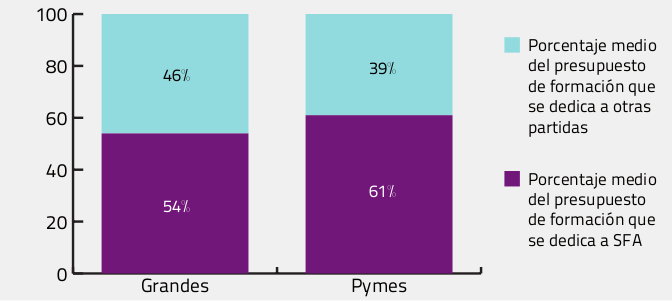
\includegraphics[width=8cm]{figs/cenatic_trainingbudget.png}
\end{center}
\end{frame}

%%%%%%%%%%%%%%%%%%%%%%%%%%%%%%%%%%%%%%%%%%%%%%%%%%%%%%%%%%%%

\begin{frame}
\frametitle{External and internal training}
\begin{itemize}
\item Clear preference for internal training
\item Usually carried out by internal experts
\item Big companies tend to this scheme 
\end{itemize}
\end{frame}

%%%%%%%%%%%%%%%%%%%%%%%%%%%%%%%%%%%%%%%%%%%%%%%%%%%%%%%%%%%%


\begin{frame}
\frametitle{External training}
\begin{center}
  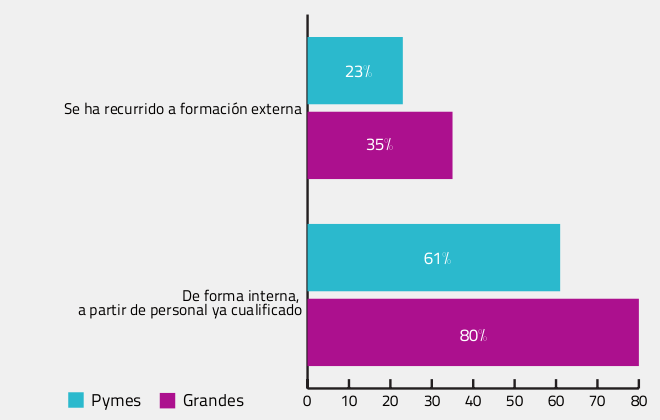
\includegraphics[width=8cm]{figs/cenatic_externaltraining.png}
\end{center}
\end{frame}

%%%%%%%%%%%%%%%%%%%%%%%%%%%%%%%%%%%%%%%%%%%%%%%%%%%%%%%%%%%%

\begin{frame}
\frametitle{Questions? / Comments?}
\begin{center}
\huge{Questions? / Comments?}
\end{center}
\end{frame}

%%%%%%%%%%%%%%%%%%%%%%%%%%%%%%%%%%%%%%%%%%%%%%%%%%%%%%%%%%%%

\end{document}
